\documentclass[11pt]{article}
\usepackage{cite}
\usepackage{fullpage}
\usepackage{ifpdf}
\ifpdf
  \usepackage{hyperref}
\else
  \usepackage[hypertex]{hyperref}
\fi
\usepackage{array}
\usepackage{times}
\usepackage{url}
\usepackage{amsmath}
\usepackage{breqn}
\usepackage{latexsym}
\usepackage{pgfplotstable}
\usepackage{algorithm2e}
\usepackage{hhline}
\usepackage{multirow}
\usepackage{caption}
\usepackage{subcaption}
\usepackage{color}
\usepackage{lipsum,adjustbox}
\usepackage{tikz}
\usepackage{tikz-dependency}
\usetikzlibrary{shapes,fit,calc,er,positioning,intersections,decorations.shapes,mindmap,trees}
\tikzset{decorate sep/.style 2 args={decorate,decoration={shape backgrounds,shape=circle,
      shape size=#1,shape sep=#2}}}

\newcommand{\secref}[1]{Section~\ref{#1}}
\newcommand{\figref}[1]{Figure~\ref{#1}}
\newcommand{\tabref}[1]{Table~\ref{#1}}
\newcommand{\algref}[1]{Algorithm~\ref{#1}}
\DeclareMathOperator*{\argmin}{argmin}
\DeclareMathOperator*{\argmax}{argmax}
\SetKwRepeat{Do}{do}{while}
\renewcommand\AlCapFnt{\normalfont\small}

\makeatletter
\renewcommand{\paragraph}{
  \@startsection{paragraph}{4}
  {\z@}{.3ex \@plus .3ex \@minus .2ex}{-1em}
  {\normalfont\normalsize\bfseries}
}

\title{Research Proposal}
\author{Daniel Hershcovich}
\date{\today \\ \textit{The Hebrew University of Jerusalem}}

\begin{document}
\maketitle

\begin{table}[!th]
\begin{tabular}{>{\bfseries}l p{0.5\textwidth}}
Supervisor & Prof. Ari Rappoport \\
Title & Universal Semantic Parsing
\end{tabular}
\end{table}


\section{Introduction}

In order to represent the full range of semantic structures exhibited by
natural language, there are three structural properties that should be supported.
The first is \textbf{multiple parents},
representing arguments and relations (semantic units) that are shared between predicates.
For instance, in the sentence
``After graduation, John moved to Paris'', ``John'' is an argument of both ``graduation''
and ``moved'', yielding a DAG structure (\figref{fig:graduation}), rather than a tree.

The second is \textbf{non-terminal nodes} for representing units
comprising more than one word.
While bi-lexical dependencies partially circumvent this requirement, by
representing complex units in terms of their headwords, they fall short
when representing units that have no clear head.
Frequent examples of such constructions include
coordination structures (e.g., ``\textit{John and Mary} went home''; \figref{fig:home}),
some multi-word expressions (e.g., ``The Haves and the \textit{Have Nots}''),
and prepositional phrases.
In these cases, dependency schemes often apply some annotation convention that selects one of the sub-units
as the head, but as different head selections are needed for different purposes,
standardization problems arise \cite{Ivanova2012who}.
For example, selecting the preposition to head prepositional phrases yields better
parsing results \cite{Schwartz:12}, while the head noun can be more useful for
information extraction purposes.

Third, semantic units may be \textbf{discontinuous} in the text. For instance, in
``John \textit{gave} everything \textit{up}''
(\figref{fig:gave}), the phrasal verb ``gave ... up'' forms a single semantic unit.
Discontinuities are also pervasive with other multi-word
expressions \cite{schneider2014discriminative}.
We call formal representations supporting all three properties 
{\it Broad-coverage Semantic Structures} (BSS).

\begin{figure}[t]
  \begin{subfigure}[t]{\columnwidth}
  \parbox{.2\textwidth}{\caption{}\label{fig:graduation}}
  \parbox{.8\textwidth}{
  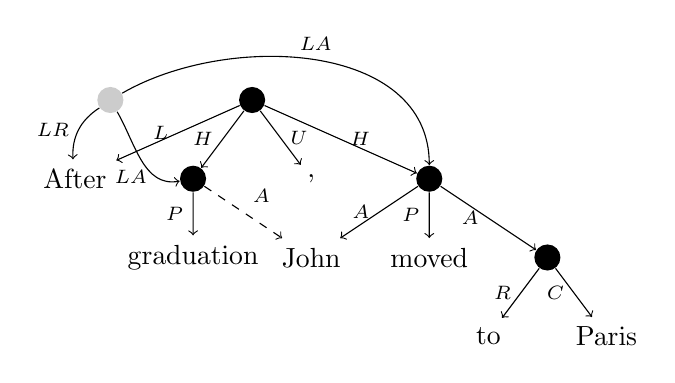
\begin{tikzpicture}[level distance=10mm, ->]
    \node (ROOT) [fill=black, circle] {}
      child {node (After) {After} edge from parent node[left] {\scriptsize $L$}}
      child {node (graduation) [fill=black, circle] {}
      {
        child {node {graduation} edge from parent node[left] {\scriptsize $P$}}
      } edge from parent node[left] {\scriptsize $H$} }
      child {node {,} edge from parent node[right] {\scriptsize $U$}}
      child {node (moved) [fill=black, circle] {}
      {
        child {node (John) {John} edge from parent node[left] {\scriptsize $A$}}
        child {node {moved} edge from parent node[left] {\scriptsize $P$}}
        child {node [fill=black, circle] {}
        {
          child {node {to} edge from parent node[left] {\scriptsize $R$}}
          child {node {Paris} edge from parent node[left] {\scriptsize $C$}}
        } edge from parent node[left] {\scriptsize $A$} }
      } edge from parent node[right] {\scriptsize $H$} }
      ;
    \draw[dashed,->] (graduation) to node [auto] {\scriptsize $A$} (John);
    \node (LKG) at (-1.8,0) [fill=black!20, circle] {};
          \draw[bend right] (LKG) to node [auto, left] {\scriptsize $LR$} (After);
          \draw (LKG) to[out=-60, in=190] node [below] {\scriptsize $LA\quad$} (graduation);
    \draw (LKG) to[out=30, in=90] node [above] {\scriptsize $LA$} (moved);
  \end{tikzpicture}
  }
  \end{subfigure}
  \begin{subfigure}[t]{\textwidth}
  \parbox{.2\textwidth}{\caption{}\label{fig:shower}}
  \parbox{.8\textwidth}{
  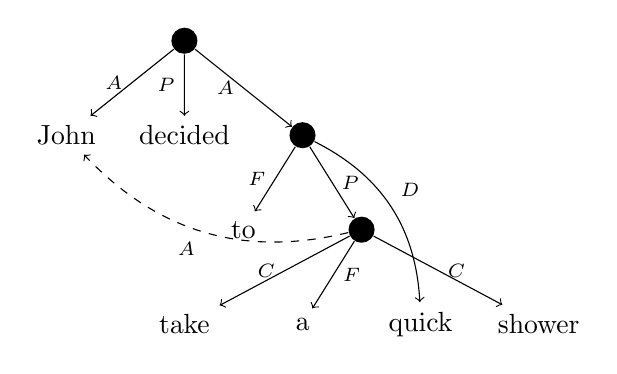
\begin{tikzpicture}[level distance=12mm, ->,
      every node/.append style={midway}]
    \node (ROOT) [fill=black, circle] {}
      child {node (John) {John} edge from parent node[left] {\scriptsize $A$}}
      child {node {decided} edge from parent node[left] {\scriptsize $P$}}
      child {node (totakeaquickshower) [fill=black, circle] {}
      {
        child {node {to} edge from parent node[left] {\scriptsize $F$}}
        child {node (takeashower) [fill=black, circle] {}
        {
          child {node {take} edge from parent node[left] {\scriptsize $C$}}
          child {node {a} edge from parent node[right] {\scriptsize $F$}}
          child {node (quick) {quick} edge from parent[white]}
          child {node {shower} edge from parent node[right] {\scriptsize $C$}}
        } edge from parent node[right] {\scriptsize $P$} }
      } edge from parent node[left] {\scriptsize $A$} }
      ;
    \draw[bend left,dashed,->] (takeashower) to node [auto] {\scriptsize $A$} (John);
    \draw[bend left,->] (totakeaquickshower) to node [auto] {\scriptsize $D$} (quick);
  \end{tikzpicture}
  }
  \end{subfigure}
  \begin{subfigure}[t]{.9\textwidth}
  \parbox{.2\textwidth}{\caption{}\label{fig:home}}
  \hspace{.1\textwidth}
  \parbox{.7\textwidth}{
  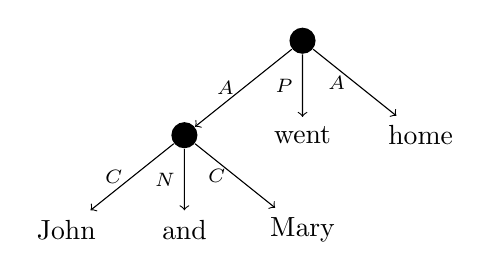
\begin{tikzpicture}[level distance=12mm, ->,
      every node/.append style={midway}]
    \node (ROOT) [fill=black, circle] {}
      child {node [fill=black, circle] {}
      {
        child {node {John} edge from parent node[left] {\scriptsize $C$}}
        child {node {and} edge from parent node[left] {\scriptsize $N$}}
        child {node {Mary} edge from parent node[left] {\scriptsize $C$}}
      } edge from parent node[left] {\scriptsize $A$} }
      child {node {went} edge from parent node[left] {\scriptsize $P$}}
      child {node {home} edge from parent node[left] {\scriptsize $A$}}
      ;
  \end{tikzpicture}
  }
  \end{subfigure}
  \begin{subfigure}[t]{.9\textwidth}
  \parbox{.2\textwidth}{\caption{}\label{fig:gave}}
  \hspace{.2\textwidth}
  \parbox{.6\textwidth}{
  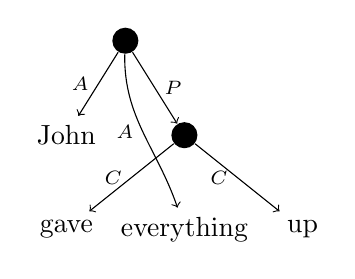
\begin{tikzpicture}[level distance=12mm, ->,
      every node/.append style={midway}]
    \node (ROOT) [fill=black, circle] {}
      child {node {John} edge from parent node[left] {\scriptsize $A$}}
      child {node [fill=black, circle] {}
      {
      	child {node {gave} edge from parent node[left] {\scriptsize $C$}}
      	child {node (everything) {everything} edge from parent[white]}
      	child {node {up} edge from parent node[left] {\scriptsize $C$}}
      } edge from parent node[right] {\scriptsize $P$} }
      ;
    \draw[bend right,->] (ROOT) to[out=-20, in=180] node [left] {\scriptsize $A$} (everything);
  \end{tikzpicture}
  }
  \end{subfigure}
  \caption{\label{fig:examples}
    Semantic representation of the three structural properties
    required for BSS, according to the UCCA scheme. (\subref{fig:graduation}) includes a remote edge (dashed),
    resulting in ``John'' having two parents. % and a linkage relation (gray node and its outgoing edges).
    (\subref{fig:home}) includes a coordination construction (``John and Mary'').
    (\subref{fig:gave}) includes a discontinuous unit (``gave ... up'').
    Legend: $P$ -- a Scene's main relation, $A$ -- participant,
    $L$ -- inter-scene linker, $H$ -- linked Scene, $C$ -- center,
    $R$ -- relator, $N$ -- connector, $U$ -- punctuation, $F$ -- function unit.
    Pre-terminal nodes are omitted for brevity.
  }
\end{figure}

However, to our knowledge, no existing parser supports the combination of these criteria.
The only semantic annotation scheme that supports them is UCCA \cite{abend2013universal},
which has no parser.
Several other models either support some of these properties \cite{oepen2015semeval},
or avoid grounding semantic units altogether
(notably, AMR \cite{banarescu2013abstract}).
\secref{sec:background} discusses these models.

In this work we are first in proposing techniques for BSS parsing.
We adopt a transition-based approach, which has recently produced some of the best
results in syntactic dependency parsing
\cite{dyer2015transition,ballesteros2015improved}, and has also demonstrated
strong performance in a variety of other semantic and syntactic settings
\cite[among others]{maier2015discontinuous,wang2015transition}.
Transition-based methods are a natural starting point for UCCA parsing,
as the set of distinctions it represents, which is centered around predicate-argument
structures and their inter-relations, is similar in spirit to the distinctions
conveyed by dependency schemes.

We pursue two complementary parsing strategies.
First, we assess the ability of existing technology to tackle the task,
by developing conversion protocols between UCCA structures and two related formalisms:
dependency trees and discontinuous constituency trees.
As these formalisms are more restrictive than BSS, the conversion
is necessarily lossy. Nonetheless, we find that it is effective
in practice (\secref{sec:conversion_approach}).
Second, we present a novel transition-based broad-coverage parser,
Broad-coverage Semantic Parser (\textsc{bsp}; \secref{sec:direct_approach})
that supports multiple parents, non-terminal nodes and discontinuous units,
based on extending existing transition-based parsers
with new transitions and features.

We experiment with the English UCCA-annotated corpora \cite{abend2013universal}
as a test case, in both in-domain and out-of-domain scenarios, reaching
nearly 70\% labeled F-score for the highest scoring parser.
The results suggest concrete paths for further improvement.

\section{Background}\label{sec:background}

\subsection{Annotation of linguistic structure}

Semantic tasks in natural language processing, such as machine translation and sentiment analysis, require understanding the meaning of text. Since text is merely a sequence of words, it has to be represented in a way that will convey its meaning. One simple approach, known as the bag-of-words model, looks only at which multi-set of words occurs in the text. This can already provide substantial information about the meaning, but it ignores the order of words, which clearly conveys important information as well. The n-gram model counts sequences of words with regard to their order, incorporating at least some of the meaning encoded in the text structure. These models and variations of them are quite successfully applied to a variety of tasks\cite{mikolov2013efficient}. Nevertheless, an undeniable part in the meaning of language resides in its hierarchical structure. Syntax is a way to model this structure formally. Using syntactic features can improve the performance in semantic tasks\cite{vandeghinste2013parse}.

However, syntactic annotations suffer from limitations, since they do not represent the semantic structure of text directly. Simple manipulations such as switching from an active construction to a passive one, which nearly do not alter the meaning of text, can yield a significantly different syntactic structure. Moreover, the same syntactic construct can express conceptually distinct semantic structures\cite{abend2013ucca}.


\paragraph{Semantic annotation}

Semantic annotation schemes attempt to represent the meaning of natural language utterances directly. An example is semantic role labeling\cite{baker1998framenet}\cite{paass2014semantic}, which annotates predicates and their arguments, classifying them into specific roles. As opposed to syntactic annotation, which reflects language-specific formal patterns, semantic annotation corresponds to a higher level of cognitive processing, and the same framework can potentially apply to any language. Moreover, a rich semantic annotation scheme may be more beneficial than syntactic annotation as an input for applications that attempt to solve a semantic task, due to their tighter relation to the meaning of the text.

Semantic parsing methods can be largely partitioned into grammar-based and grammarless methods.
Within the grammar-based literature, most work relied on Combinatory Categorial Grammar (CCG)
\cite{Steedman:00}, which allows computing semantic structure compositionally from the
syntactic derivations. Notable examples include the Boxer parser \cite{bos2005towards}
and the AMR parser by \cite{artzi2015broad}.
Other examples include parsing with Hyperedge Replacement Grammars
\cite{jones2012semantics,chiang2013parsing,peng2015synchronous} and
graph grammars \cite{koller2015semantic}.
A different line of work takes a discriminative, grammarless approach,
pursuing either graph-based methods that predict the highest ranking graph
(tree or DAG) that satisfies a given set of constraints
\cite[for AMR parsing]{flanigan2014discriminative}.
or a transition-based method that builds the parse incrementally following a series of local
decisions \cite[and much subsequent work]{Nivre03anefficient}.

\paragraph{Broad-coverage Semantic Representation.}
While earlier work on semantic parsing has mostly concentrated on shallow semantic analysis,
focusing on semantic role labeling of verbal argument structures,
the focus has recently shifted to parsing of more elaborate representations that account
for a wider range of phenomena. 
Most closely related to this work is Broad-coverage Semantic Dependency Parsing (SDP),
addressed in two SemEval tasks \cite{oepen2014semeval,oepen2015semeval},
experimenting with the Prague tectogrammatical layer \cite{sgallhp:1986,bohmova2003prague},
and with dependencies derived from the Enju parser\footnote{See \url{http://kmcs.nii.ac.jp/enju/}.}, and Lingo ERG \cite{Flic:02}.
Like BSS parsing, SDP addresses a wide range of semantic phenomena,
and supports discontinuous units and multiple parents. However, SDP uses
bi-lexical dependencies, disallowing non-terminal nodes, and thus faces difficulties in supporting
structures that have no clear head, such as coordination \cite{Ivanova2012who}.

Another line of work addresses parsing into Abstract Meaning Representations (AMRs)
\cite{flanigan2014discriminative,vanderwende2015amr,pust2015parsing,artzi2015broad}. 
While sharing much of this work's motivation,
AMR does not ground its units in the words and constituents of the text.
This complicates the parsing task, as it requires
that the alignment between words and logical symbols be automatically
(and imprecisely) detected.
\cite{wang2015transition} applied a transition-based approach to AMR parsing,
but their method involved first syntactically parsing the input, and then converting
the resulting tree into an AMR. They thus used a different set of transitions than
\textsc{bsp}, which parses strings directly into graphs.


\paragraph{UCCA Annotation Scheme.}
Universal Cognitive Conceptual Annotation (UCCA)
is a cross-linguistically applicable semantic representation scheme,
that builds on the established ``Basic Linguistic Theory'' framework for typological description
\cite{Dixon:10b,Dixon:10a,Dixon:12}, and on the Cognitive Linguistics literature.
UCCA is a multi-layered representation, where each layer corresponds to a ``module'' of
semantic distinctions (e.g., predicate-argument structures, adverbials, coreference etc.).
%Importantly, the same set of categories can be applied across different lexical items and languages.
%This stands in contrast to more schemes such as FrameNet \cite{Baker:98},
%PropBank \cite{Palmer:05} and AMR, that define an open-ended, lexically-based set of categories,
%which while providing further information, are more prone to coverage issues \cite{Palmer:10},
%and may result in a different set of relations when applied to different languages \cite{Xue2014not}.

Formally, a UCCA structure over a sentence is a DAG, whose leaves correspond to the sentence's words.
The nodes of the graph, or its ``units'', are either terminals or several
sub-units (not necessarily contiguous) jointly viewed as a
single entity according to some semantic or cognitive consideration.
Edges bear a category, indicating the role of the sub-unit in the relation that the parent represents.
UCCA structures support all three criteria of BSS: multiple parents, non-terminal nodes, and
discontinuous units.

UCCA's foundational layer, which we use here, covers the predicate-argument
structures evoked by predicates of all grammatical categories
(verbal, nominal, adjectival and others), the inter-relations between them,
as well as other major linguistic phenomena such as coordination and multi-word expressions.
This set of categories has demonstrated applicability to multiple languages, including
English, French, German and Czech, support for rapid annotation, and semantic stability in translation:
UCCA annotations of translated text usually contain the same set of relationships
\cite{sulem2015conceptual}. This finding supports the claim that UCCA represents an abstract
level of semantics, shared by different languages.

The layer's basic notion is the {\it Scene}, which describes a movement, an action or a state.
Each Scene contains one Main Relation, as well as one or more Participants.
For example, the sentence ``After graduation, John moved to Paris'' contains two Scenes,
whose main relations are ``graduation'' and ``moved''. ``John'' is a Participant in both Scenes,
while ``Paris'' only of the latter.
We note that the scheme marks one of the incoming edges for each non-root
as ``primary'' and the others as ``remote'' edges.
The two Scenes in this sentence are both arguments of the \textit{Linker} ``After'',
which in this case expresses a temporal relation between them.
\figref{fig:examples} presents the UCCA annotation of this and other examples.

Further categories account for relations between Scenes and the internal structures of
complex arguments (e.g., coordination) and relations
(e.g., complex adverbials, such a ``very clearly''). UCCA graphs may contain implicit
units that have no correspondent in the text, but the parsing of these
units is deferred to future work, as it is likely to require different methods
than those explored here \cite{roth2015inducing}.


% TODO incorporate this or delete it:
Universal Conceptual Cognitive Annotation (UCCA) is a recently introduced semantic annotation scheme \cite{abend2013ucca}\cite{abend2013universal}. This scheme takes a semantic approach to grammatical representation, describing relations between words and phrases in the whole text. It has a coarse foundational layer that can be extended by any number of additional layers to provide more refinements and sophistication, but it already covers the most important semantic relations in language, including verb-argument structure, adjuncts, clause embeddings and linkage. The text is represented by a graph structure, where the edges denote semantic dependencies. The foundational layer contains 12 such relations. The scheme is motivated and justified by Cognitive Linguistics theories that provide a theoretical framework for the semantic structure of language, supported by cross-linguistic evidence.

Being a semantic scheme, UCCA is close to the human cognitive processing of language. Therefore, it is easy for human annotators to grasp, and does not require expertise in linguistics or long training. A corpus containing 160K words from the English Wikipedia has been manually annotated with the foundational layer\footnote{\url{http://www.cs.huji.ac.il/~oabend/ucca.html}}.

A key idea in the basis of the UCCA project is to use manual annotation for supervised learning of semantic distinctions that are natural for human annotators, while inducing distributional regularities from text in an unsupervised manner.

\figref{fig:soybeans} shows the UCCA annotation for the sentence
``A similar technique is almost impossible to apply to other crops, such as cotton, soybeans and rice.''.
The sentence was used by \cite{oepen2015semeval} to compare between the difference schemes.
It includes a single Scene, whose main relation is ``apply'', a secondary relation ``almost impossible'', as well as two complex arguments: ``a similar technique'' and the coordinated argument ``such as cotton, soybeans, and rice.''

\begin{figure}
  \centering
  \scalebox{.6}{
  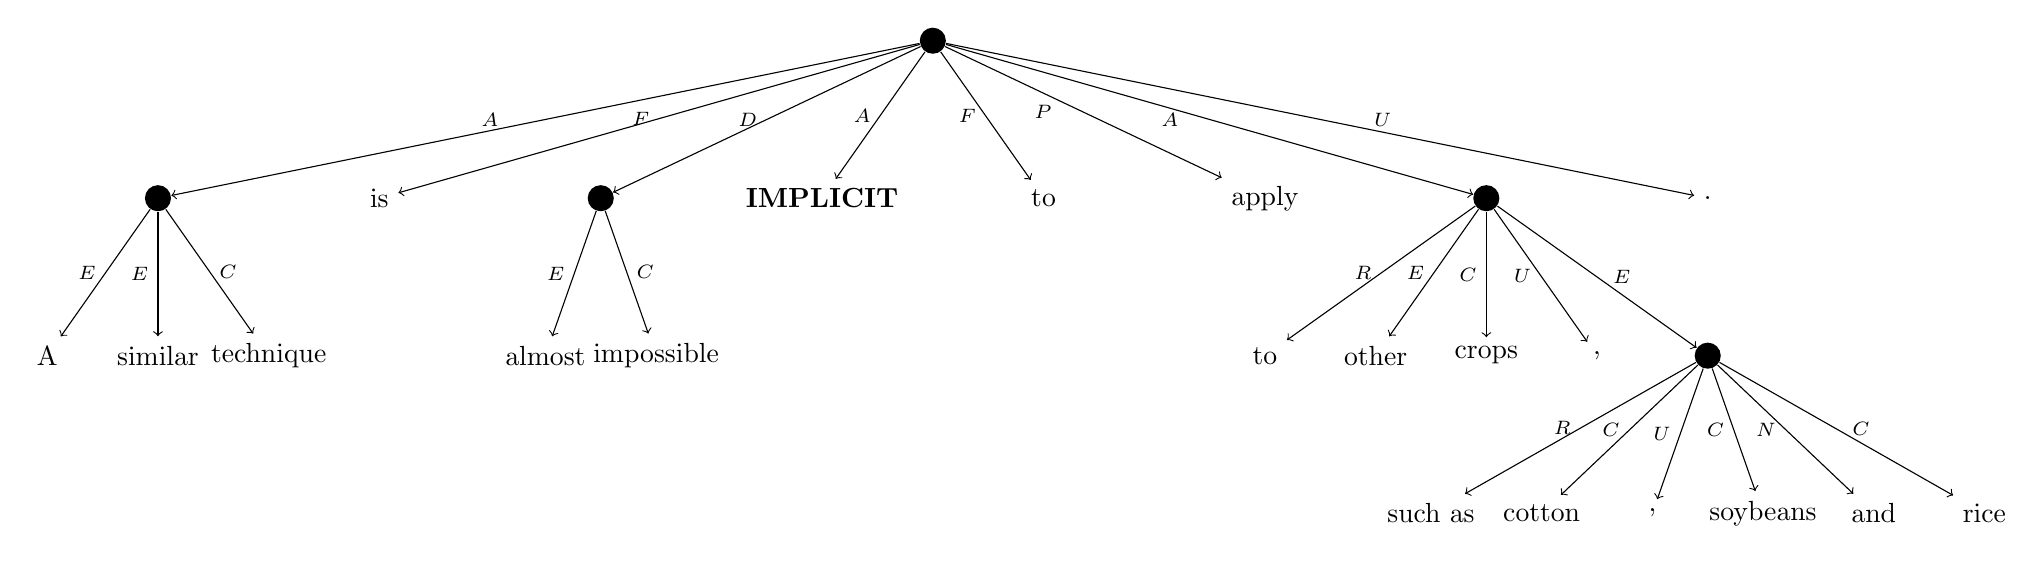
\begin{tikzpicture}[level distance=20mm, ->,
  level 1/.style={sibling distance=8em},
  level 2/.style={sibling distance=4em},
  level 3/.style={sibling distance=4em}]
    \node (ROOT) [fill=black, circle] {}
      child {node [fill=black, circle] {}
      {
        child {node {A} edge from parent node[left] {\scriptsize $E$}}
        child {node {similar} edge from parent node[left] {\scriptsize $E$}}
        child {node {technique} edge from parent node[right] {\scriptsize $C$}}
      } edge from parent node[left] {\scriptsize $A\quad$ \hspace{1mm} } }
      child {node {is} edge from parent node[left] {\scriptsize $F$}}
      child {node [fill=black, circle] {}
      {
        child {node {almost} edge from parent node[left] {\scriptsize $E$}}
        child {node {impossible} edge from parent node[right] {\scriptsize $C$}}
      } edge from parent node[left] {\scriptsize $D$} }
      child {node {\textbf{IMPLICIT}} edge from parent node[left] {\scriptsize $A$}}
      child {node {to} edge from parent node[left] {\scriptsize $F$}}
      child {node {apply} edge from parent node[left] {\scriptsize $P\quad$}}
      child {node [fill=black, circle] {}
      {
        child {node {to} edge from parent node[left] {\scriptsize $R$}}
        child {node {other} edge from parent node[left] {\scriptsize $E$}}
        child {node {crops} edge from parent node[left] {\scriptsize $C$}}
        child {node {,} edge from parent node[left] {\scriptsize $U$}}
        child {node [fill=black, circle] {}
        {
          child {node {such as} edge from parent node[left] {\scriptsize $R$}}
          child {node {cotton} edge from parent node[left] {\scriptsize $C$}}
          child {node {,} edge from parent node[left] {\scriptsize $U$}}
          child {node {soybeans} edge from parent node[left] {\scriptsize $C$}}
          child {node {and} edge from parent node[left] {\scriptsize $N$}}
          child {node {rice} edge from parent node[right] {\scriptsize $\; C$}}
        } edge from parent node[right] {\scriptsize $\; E$ \hspace{1mm} } }
      } edge from parent node[left] {\scriptsize $A\;$ \hspace{1mm} } }
      child {node {.} edge from parent node[right] {\scriptsize $\quad \quad U$}}
      ;
  \end{tikzpicture}
  }
  \caption{Additional UCCA example
  \label{fig:soybeans}
  }
\end{figure}


\subsection{Deep neural networks}

Deep learning in artificial neural networks has received much attention in several fields of computer science, including computer vision, speech recognition and natural language processing, due to their best performance in various tasks\cite{collobert2011nlp}.


\subsubsection{Distributed representation}

In natural language processing, many of the deep learning methods rely strongly on representation of words as vectors in a continuous vector space with tens or hundreds of dimensions\cite{turian2010word}, such that linguistic and semantic regularities between the words are captured in the vectors\cite{mikolov2013linguistic}. This kind of representation, called \textit{word embedding}, can be learned in an unsupervised manner, from a large unlabeled corpus.

Several models have been suggested to learn distributed representations for phrases, based on the representations for single words. Recursive neural networks (see~\ref{subsec:rnns}) can learn semantically meaningful continuous vector representations of multi-word phrases and sentences, typically in the same space as the word embedding, using supervised training for structure prediction\cite{socher2010learning}. They have achieved state-of-the-art performance on paraphrase detection, sentiment analysis, relation classification, syntactic parsing, image-sentence mapping, and knowledge base completion, among other tasks\cite{socher2013parsing}\cite{socher2013recursive}. This model is one of the first attempt for structure prediction using deep learning. Recurrent neural networks can also learn phrase representations, and they have a relatively simple model that does not depend on pre-annotation of structure.



\section{Previous work}

Supervised learning of a simplification of UCCA has already been attempted by flattening the structure, to get a sequence tagging problem\cite{beka2013thesis}. An accuracy of $65\%$ was achieved using a maximum-entropy model. After these initial results, however, the task was abandoned, firstly because the data set was still small at the time (only a few thousands of words), and secondly due to the realization that further conversion from a flat tagging scheme to the full hierarchic one is not trivial, and could cause subsequent error in the annotation. Therefore, a direct hierarchic structure prediction may be more reliable. Some attempts were made at a partial rule-based heuristic approach, but they proved inefficient. On the identification of scene-evoking nouns, a subset of a specific type of relation in UCCA, the performance was not very high either.



\section{Aims}

In my research, I intend on pursuing the following goals:

\begin{itemize}
  \item Devising a method for automatic prediction of the UCCA structure, including at least the foundational layer and possibly more refinements when they are defined. In general, developing a method for deep learning of DAG dependency structures, which would be a very useful novelty.
  \item Evaluating the distributed representation that is learned in the process of training a deep learning model on the UCCA task, and investigating whether it reflects the semantic similarity and relatedness between phrases better than the representation learned while training a network for the prediction of a syntactic structure.
  \item Using the new automatic annotation to improve the performance of existing techniques for solving semantic tasks, such as sentiment analysis and machine translation, that are currently mostly based on syntactic parsing or simpler structures for the representation of text compositionality.
\end{itemize}



\section{Methods}

\subsection{Conversion-Based Parsing}\label{sec:conversion_approach}

We begin by assessing the ability of existing technology to address the task,
by taking a conversion-based approach. Training proceeds by 
converting BSS into a different representation,
and training an existing parser on the converted structures.
We evaluate the trained parsers by applying them to the test set,
and converting the results back to BSS, where they are compared
with the gold standard.
The error resulting from this back and forth conversion is discussed in
\secref{sec:results}.

\paragraph{Notation.}
Let $L$ be the set of possible edge labels.
A BSS is a directed acyclic graph $G=(V,E, \ell)$
over a sequence of tokens $w_1, \ldots, w_n$,
where $\ell:E\to L$ is a function of \textit{edge labels}.
For each token $w_i$ ($i=1, \ldots, n$), there exists a leaf (or a terminal) $t_i \in V$.

\paragraph{Conversion to Constituency Trees.}
We convert BSS to constituency trees by removing a subset of the
edges\footnote{For trees, labeling nodes is equivalent to labeling edges. Thus,
  we do not distinguish between the two options. 
  Note also that as the original structures may contain discontinuities, so may the resulting trees.}.
Specifically, when converting UCCA structures, we simply remove all remote edges,
leaving only primary edges, which form a tree structure (see \figref{fig:graduation}).
The inverse conversion from trees to BSS is simply the identity function, as every constituency tree is a BSS.

\paragraph{Conversion to Dependency Trees.}\label{subsec:con2dep}
In the conversion to dependency trees, we first convert BSS
to constituency trees using the above procedure, and then convert the result to dependency trees. 
Assume $T_c=(V_c,E_c,\ell_c)$ is a constituency tree with labels $\ell_c:E_c~\rightarrow~L$,
where $L$ is the set of possible labels.
The conversion from $T_c$ to a dependency tree involves the removal of
all non-terminals from $T_c$ and the addition of edges between terminals.
The nodes of the converted dependency tree are simply the terminals of $T_c$.

We define a linear order over possible edge labels $L$.
For each node $u \in V$, denote with $h(u)$ its child with the highest edge label.
Denote with $h^*(u)$ the terminal reached by recursively applying $h(\cdot)$ over $u$.
For each terminal $t$, we define $n(t)$ as the highest
non-terminal such that $t=h^*(n(t))$, i.e.,
$n(t)$ is the only node such that $t=h^*(n(t))$ and $t \neq h^*(\mathrm{Parent}_c(n(t)))$.
The head of $t$ according to the dependency graph is
the terminal $h^*(\mathrm{Parent}_c(n(t)))$.
The complete conversion procedure from constituency to dependency is given in \algref{alg:con2dep}.

We note that this conversion procedure is simpler than the
head percolation procedure used for converting syntactic constituency
trees to dependency trees.
This is because $h(u)$ of a node $u$ (similar to $u$'s head-containing child),
depends only on the label of the edge $(h(u),u)$, and not on the sub-tree spanned by $u$,
because edge labels in UCCA directly express the role of the child in the parent unit, and
are thus sufficient for determining which of $u$'s children contains the head node.
%This is appropriate, since edges in a semantic constituency graph express the relation between units,
%whereas in syntactic constituency trees the identity of a node depends on the nodes below it.

\begin{algorithm}[t]
  \small
  \KwData{constituency tree ${T_c}=(V_c,E_c,\ell_c)$}
 \KwResult{dependency tree $T_d=(V_d,E_d,\ell_d)$}
 \ForEach{$u \in V_c$} {
  $h(u) \leftarrow \argmin_v \mathrm{Priority}(\ell_c(u,v))$\;
 }
 $V_d \leftarrow \mathrm{Terminals}({T_c})$,
 $E_d \leftarrow \emptyset$\;
 \ForEach{$t \in V_d$} {
  $u \leftarrow t$\;
  \While{$u=h(\mathrm{Parent}_c(u))$} {
  	$h^*(u) \leftarrow t$\;
  	$u \leftarrow \mathrm{Parent}_c(u)$\;
  }
  $n(t) \leftarrow h(u)$\;
 }
 \ForEach{$t \in V_d$} {
  $u \leftarrow \mathrm{Parent}_c(n(t))$\;
  $t^\prime \leftarrow h^*(u)$\;
  $E_d \leftarrow E_d \cup \{(t^\prime, t)\}$\;
  $\ell_d (t^\prime, t) \leftarrow \ell_c(u, n(t))\}$\;
 }
 \caption{Constituency to dependency conversion procedure.}
 \label{alg:con2dep}
\end{algorithm}

The order of labels defines as the $\mathrm{Priority}$ function in \algref{alg:con2dep} is the following:

\begin{enumerate}
\item $C$ (\textit{Center})
\item $N$ (\textit{Connector})
\item $H$ (\textit{ParallelScene})
\item $P$ \textit{Process})
\item $S$ (\textit{State})
\item $A$ (\textit{Participant})
\item $D$ (\textit{Adverbial})
\item $T$ (\textit{Time})
\item $E$ (\textit{Elaborator})
\item $R$ (\textit{Relator})
\item $F$ (\textit{Function})
\item $L$ (\textit{Linker})
\item $LR$ (\textit{LinkRelation})
\item $LA$ (\textit{LinkArgument})
\item $G$ (\textit{Ground})
\item $\mathit{Terminal}$ (\textit{Terminal})
\item $U$ (\textit{Punctuation})
\end{enumerate}

The inverse conversion introduces non-terminal nodes back into the tree.
As the distinction between low- and high-attaching nodes is lost in the constituency to
dependency conversion, we heuristically assume that attachments are always
high-attaching.
Assume $T_d=(V_d,E_d,\ell_d)$ is a dependency tree.
We begin by creating a root node $r$.
Then, iterating over $V_d$ in topological order,
we add its members as terminals to the constituency tree
and create a pre-terminal parent for each,
with an edge labeled as \textit{Terminal} between them.
The parents of the pre-terminals are determined by the terminal's parent in the dependency
tree: if a dependency node $t$ is a child of the root in $T_d$, then $t$'s pre-terminal will also be a child of the root node. Otherwise, $t$'s pre-terminal is the child of the pre-terminal associated with $t$'s head in $T_d$. We add an intermediate node in between if $t$ has any dependents in $T_d$,
to allow adding their pre-terminals as children.
Edge labels for the intermediate edges are determined by a rule-based function, denoted by $\mathrm{Label}(u)$:
see \algref{alg:dep2con}.
In practice, it mostly selects the UCCA label \textit{Center}.
The conversion procedure from dependency to constituency is given in \algref{alg:dep2con}.

\begin{algorithm}[t]
  \small
 \KwData{dependency tree $T_d=(V_d,E_d,\ell_d)$}
 \KwResult{constituency tree $T_c=(V_c,E_c,\ell_c)$}
 $r \leftarrow \mathrm{Node()}$\;
 $V_c \leftarrow \{r\}$,
 $E_c \leftarrow \emptyset$\;
 \ForEach{$t \in \mathrm{TopologicalSort}(V_d)$} {
  $u \leftarrow \mathrm{Node()}$\;
  $V_c \leftarrow V_c \cup \{u, t\}$\;
  $E_c \leftarrow E_c \cup \{(u, t)\}$\;
  $\ell_c(u,t)\leftarrow\mathit{Terminal}$\;
  $t^\prime \leftarrow \mathrm{Parent}_d(t)$\;
  \eIf{$t^\prime = \textsc{Root}$} {
   $E_c \leftarrow E_c \cup \{(r, u)\}$\;
   $\ell_c(r, u) \leftarrow \mathrm{Label}(r)$\;
  } {
   \eIf{$\exists v \in V_d : (t,v) \in E_d$} {
    $u^\prime \leftarrow \mathrm{Node()}$\;
    $E_c \leftarrow E_c \cup \{(u^\prime, u)\}$\;
    $\ell_c(u^\prime, u) \leftarrow \mathrm{Label}(u^\prime)$\;
   } {
    $u' \leftarrow u$\;
   }
   $p \leftarrow \mathrm{Parent}_c(t^\prime)$\;
   $E_c \leftarrow E_c \cup \{(p, u^\prime)\}$\;
   $\ell_c(p, u^\prime) \leftarrow \ell_d(t^\prime, t)$\;
  }
 }
 \caption{Dependency to constituency conversion procedure.}
 \label{alg:dep2con}
\end{algorithm}

\begin{algorithm}[ht]
  \small
  \KwData{node $u \in V_d$}
 \KwResult{label $\ell \in L$}
 \uIf{$\mathrm{IsPunctuation}(u)$}{
  \Return \textit{Punctuation}\;
 }
 \uElseIf{$\exists v \in V_d : \ell(u,v) = \textit{ParallelScene}$}{
  \Return \textit{ParallelScene}\;
 }
 \uElseIf{$\exists v \in V_d : \ell(u,v) = \textit{Participant}$}{
  \Return \textit{Process}\;
 }
 \uElse{
  \Return \textit{Center}\;
 }
 \caption{Algorithm for the $\mathrm{Label}$ function.
 \label{alg:label}
 }
\end{algorithm}

Converting the sentence in \figref{fig:graduation} to a constituency tree consists of simply removing the remote edge:

\begin{figure}[h]
  \centering
  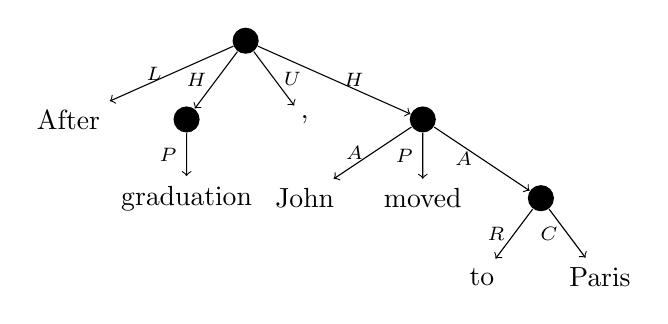
\begin{tikzpicture}[level distance=10mm, ->]
    \node (ROOT) [fill=black, circle] {}
      child {node (After) {After} edge from parent node[left] {\scriptsize $L$}}
      child {node (graduation) [fill=black, circle] {}
      {
        child {node {graduation} edge from parent node[left] {\scriptsize $P$}}
      } edge from parent node[left] {\scriptsize $H$} }
      child {node {,} edge from parent node[right] {\scriptsize $U$}}
      child {node (moved) [fill=black, circle] {}
      {
        child {node (John) {John} edge from parent node[left] {\scriptsize $A$}}
        child {node {moved} edge from parent node[left] {\scriptsize $P$}}
        child {node [fill=black, circle] {}
        {
          child {node {to} edge from parent node[left] {\scriptsize $R$}}
          child {node {Paris} edge from parent node[left] {\scriptsize $C$}}
        } edge from parent node[left] {\scriptsize $A$} }
      } edge from parent node[right] {\scriptsize $H$} }
      ;
  \end{tikzpicture}
\end{figure}

The corresponding dependency tree is given in the following figure:

\begin{figure}[h]
\centering
\begin{dependency}[theme = simple]
\begin{deptext}[column sep=.7em,ampersand replacement=\^]
After \^ graduation \^ , \^ John \^ moved \^ to \^ Paris \\
\end{deptext}
\depedge{2}{1}{L}
\depedge{2}{3}{U}
\depedge{5}{4}{A}
\depedge{2}{5}{H}
\depedge{7}{6}{R}
\depedge{5}{7}{A}
\end{dependency}
\end{figure}

\subsection{Transition-Based Broad-Coverage Semantic Parsing}\label{sec:direct_approach}

We now turn to presenting \textsc{bsp},
a transition-based parser that supports the three criteria of broad-coverage
semantic structures.

Transition-based parsing \cite{Nivre03anefficient} creates the parse
as it scans the text from left to right.
The parse is created incrementally by applying a \textit{transition} at each step to the parser state,
defined using three data structures: a buffer $B$ of tokens and nodes to be processed,
a stack $S$ of nodes currently being processed,
and a graph $G=(V,E,\ell)$ of constructed nodes and labeled edges.
Some of the states are marked as \textit{terminal}, meaning that $G$ is the final output.
A classifier is used at each step to select the next transition based on features
that encode the parser's current state.
During training, an oracle creates training instances for the classifier,
based on the gold-standard annotation.

Despite being based on local decisions, transition-based methods have yielded excellent
results in a variety of parsing tasks.
Within syntactic dependency parsing, transition-based methods
have been successfully applied to corpora in many languages and domains, yielding some
of the best reported results \cite{dyer2015transition,ballesteros2015improved}. 
The approach has also yielded results comparable with the state-of-the-art in
constituency parsing \cite{sagae2005classifier,zhang2009transition,zhu2013fast},
discontinuous constituency parsing \cite{maier2015discontinuous},
as well as dependency DAG structures
\cite{sagae2008shift,tokgoz2015transition}, CCG structures \cite{ambati2015incremental}
and AMR parsing \cite{wang2015transition}.

\textsc{bsp} mostly builds on recent advances in discontinuous constituency
and dependency DAG parsing techniques, and further introduces novel UCCA-oriented features for parsing BSS.

\paragraph{Transition Set.}
Given a sequence of tokens $w_1, \ldots, w_n$, we predict a BSS $G$ whose leaves
correspond to the tokens. % $w_1, \ldots, w_n$.
Parsing starts with a single node on the stack (the root node), and the input tokens
$w_1, \ldots, w_n$ in the buffer. The set of transitions is given in \figref{fig:transitions}.
In addition to the standard \textsc{Shift} and \textsc{Reduce} operations, 
we follow previous work in transition-based constituency parsing \cite{sagae2005classifier}, and include the \textsc{Node} transition for creating new non-terminal nodes.
Concretely, \textsc{Node$_X$} creates a new node on the buffer as a parent of the first element on the stack, with an $X$-labeled edge.


\begin{figure}
\begin{adjustbox}{width=.98\textwidth,margin=3pt,frame}
\begin{tabular}{llll|l|llllc|c}
\multicolumn{5}{c|}{\textbf{\small Initial State}} & \multicolumn{6}{c}{\textbf{\small Final State}} \\
\textbf{\footnotesize Stack} & \textbf{\footnotesize Buffer} & \textbf{\footnotesize Nodes} & \multicolumn{1}{l}{\textbf{\footnotesize Edges}} & \multicolumn{1}{c|}{\textbf{\footnotesize Terminal?}} & \textbf{\footnotesize Stack} & \textbf{\footnotesize Buffer} & \textbf{\footnotesize Nodes} & \textbf{\footnotesize Edges} & \multicolumn{1}{c}{\textbf{\footnotesize Terminal?}} \\
$[\mathrm{root}]$ & $w_{1:n}$ & \multirow{2}{40pt}{$\{\mathrm{root}\} \cup w_{1:n}$} & \multicolumn{1}{l}{$\emptyset$} & \multicolumn{1}{c|}{$-$} & $\emptyset$ & $\emptyset$ & $V$ & $E$ & \multicolumn{1}{c}{$+$} \\ 
\multicolumn{5}{c|}{} \\
\multicolumn{5}{c|}{} \\
\hline
%\end{tabular}
%\end{adjustbox}
%\begin{adjustbox}{width=\textwidth,frame}
%\begin{tabular}{llll|l|llllc|l}
\multicolumn{4}{c|}{\textbf{\small Before Transition}} & \textbf{\small Transition} & \multicolumn{5}{c|}{\textbf{\small After Transition}} & \textbf{\small Condition} \\
\textbf{\footnotesize Stack} & \textbf{\footnotesize Buffer} & \textbf{\footnotesize Nodes} & \textbf{\footnotesize Edges} & & \textbf{\footnotesize Stack} & \textbf{\footnotesize Buffer} & \textbf{\footnotesize Nodes} & \textbf{\footnotesize Edges} & \textbf{\footnotesize Terminal?} & \\
$S$ & $x \;|\; B$ & $V$ & $E$ & \textsc{Shift} & $S \;|\; x$ & $B$ & $V$ & $E$ & $-$ & \\
$S \;|\; x$ & $B$ & $V$ & $E$ & \textsc{Reduce} & $S$ & $B$ & $V$ & $E$ & $-$ & \\
$S \;|\; x$ & $B$ & $V$ & $E$ & \textsc{Node$_X$} & $S \;|\; x$ & $y \;|\; B$ & $V \cup \{ y \}$ & $E \cup \{ (y,x)_X \}$ & $-$ &
$x \neq \mathrm{root}$ \\
%$S \;|\; x$ & $B$ & $V$ & $E$ & \textsc{Implicit$_X$} & $S \;|\; x$ & $y^* \;|\; B$ & $V \cup \{ y^* \}$ & $E \cup \{ (x,y^*)_X \}$ & $-$ &
%$x \not\in w_{1:n}$ \\
$S \;|\; y,x$ & $B$ & $V$ & $E$ & \textsc{Left-Edge$_X$} & $S \;|\; y,x$ & $B$ & $V$ & $E \cup \{ (x,y)_X \}$ & $-$ &
\multirow{4}{50pt}{\vspace{-5mm}\[\left\{\begin{array}{l}
x \not\in w_{1:n},\\
y \neq \mathrm{root},\\
y \not\leadsto_G x
\end{array}\right.\]} \\
$S \;|\; x,y$ & $B$ & $V$ & $E$ & \textsc{Right-Edge$_X$} & $S \;|\; x,y$ & $B$ & $V$ & $E \cup \{ (x,y)_X \}$ & $-$ & \\
$S \;|\; y,x$ & $B$ & $V$ & $E$ & \textsc{Left-Remote$_X$} & $S \;|\; y,x$ & $B$ & $V$ & $E \cup \{ (x,y)_X^* \}$ & $-$ & \\
$S \;|\; x,y$ & $B$ & $V$ & $E$ & \textsc{Right-Remote$_X$} & $S \;|\; x,y$ & $B$ & $V$ & $E \cup \{ (x,y)_X^* \}$ & $-$ & \\
$S \;|\; x,y$ & $B$ & $V$ & $E$ & \textsc{Swap} & $S \;|\; y$ & $x \;|\; B$ & $V$ & $E$ & $-$ &
$\mathrm{i}(x) < \mathrm{i}(y)$ \\
$[\mathrm{root}]$ & $\emptyset$ & $V$ & $E$ & \textsc{Finish} & $\emptyset$ & $\emptyset$ & $V$ & $E$ & $+$ & \\
\end{tabular}
\end{adjustbox}
\caption{\label{fig:transitions}
  The transition set of \textsc{bsp}. %Following standard practice,
  We write the stack with its top to the right and the buffer with its head to the left.
  $(\cdot,\cdot)_X$ denotes a primary $X$-labeled edge, and $(\cdot,\cdot)_X^*$ a remote $X$-labeled edge.
  $\mathrm{i}(x)$ is a running index for the created nodes.
  \textsc{Edge} transitions have an additional condition: the prospective child may not
  already have a primary parent.
}
\end{figure}

%\textsc{Implicit$_X$} acts similarly, but the created node is a child instead,
%and is marked as \textit{implicit}, representing a unit that does not appear explicitly in the text.

\textsc{Left-Edge$_X$} and \textsc{Right-Edge$_X$} create a new primary $X$-labeled edge between the first two elements on the stack, where the parent is the left or the right node, respectively. As a UCCA node may only
have one incoming primary edge, \textsc{Edge} transitions are disallowed where the child node already
has an incoming primary edge.
\textsc{Left-Remote$_X$} and \textsc{Right-Remote$_X$} do not have this restriction, and the created edge is
marked as \textit{remote}. We distinguish between these two pairs of transitions, for the parser
to be able to determine whether an edge is a primary or a remote one.
In order to support the prediction of multiple parents, node and edge transitions do not automatically
apply \textsc{Reduce}. This is in line with other work on
transition-based DAG dependency parsing \cite{sagae2008shift,tokgoz2015transition}.
Once all edges for a particular node have been created, it is removed from the stack
by applying \textsc{Reduce}.

\textsc{Swap} allows handling discontinuous nodes, by popping the second
node on the stack and adding it to the top of the buffer, as with the similarly
named transition in previous work \cite{nivre2009non,maier2015discontinuous}.
Finally, \textsc{Finish} pops the root node and marks the state as terminal.

\paragraph{Features.}
\label{subsec:features}

\figref{fig:features} presents the feature templates used by the parser.
For some of the features, we used the notion of \textit{head word},
defined by the $h^*(\cdot)$ function (\secref{subsec:con2dep}).
While head words are not explicitly represented in the UCCA scheme, these
features proved useful as means of encoding word-to-word relations.

In addition to the binary features defined by the feature templates,
we employ a real-valued feature, \textbf{ratio}, corresponding to the ratio between the number of terminals to number of nodes
in the graph $G$. This novel feature serves as a regularizer for the creation of new nodes, and should be beneficial for other transition-based constituency parsers too.
Features are generally adapted from the related parsers of \cite{zhang2009transition,zhu2013fast,tokgoz2015transition,maier2015discontinuous}, with a small additional set of features encoding relevant information
for the novel \textsc{Left-Remote$_X$} and \textsc{Right-Remote$_X$} transitions.

% and \textsc{Implicit$_X$}

%$s_i$ and $b_i$ stand for the $i$th stack and buffer items respectively, $w$ stands for the head word, $t$ for its POS tag, $e$ for the head incoming edge label. Note that $e$ replaces $c$ (consituent label) from Maier~\shortcite{maier2015discontinuous}, since in UCCA the labels are on the edges rather than the units; and a unit may have more than one incoming edge. $l$ and $r$ ($ll$ and $rr$) represent the leftmost and rightmost children (grand-children) of the element; $u$ handles the unary case.
%Concerning the separator features, $p$ is a unique separator feature between the head words of $s_0$ and $s_1$; $q$ is the count of any separator features between them.
%$x$ denotes the gap type of a subgraph. There are three possible values, either "none" (fully continuous), "pass" (there is a gap at the root, i.e., this gap must be filled later further up in the graph), or "gap" (the root of this graph fills a gap, i.e., its children have gaps, but the root does not). Finally, $y$ is the sum of all gap lengths.

% FEATURES
\begin{figure}
\begin{adjustbox}{width=.98\textwidth,margin=3pt,frame}
\begin{tabular}{>{\small}l}
\begin{subfigure}[t]{.5\textwidth}
{\footnotesize Features from \cite{zhang2009transition}:} \\
\textbf{unigrams} \\
$s_0te, s_0we, s_1te, s_1we, s_2te, s_2we, s_3te, s_3we,$ \\
$b_0wt, b_1wt, b_2wt, b_3wt,$ \\
$s_0lwe, s_0rwe, s_0uwe, s_1lwe, s_1rwe, s_1uwe$ \\
\textbf{bigrams} \\
$s_0ws_1w, s_0ws_1e, s_0es_1w, s_0es_1e, s_0wb_0w, s_0wb_0t,$ \\
$s_0eb_0w, s_0eb_0t, s_1wb_0w, s_1wb_0t, s_1eb_0w, s_1eb_0t,$ \\
$b_0wb_1w, b_0wb_1t, b_0tb_1w, b_0tb_1t$ \\
\textbf{trigrams} \\
$s_0es_1es_2w, s_0es_1es_2e, s_0es_1eb_0w, s_0es_1eb_0t,$ \\
$s_0es_1wb_0w, s_0es_1wb_0t, s_0ws_1es_2e, s_0ws_1eb_0t$ \\
\textbf{separator} \\
$s_0wp, s_0wep, s_0wq, s_0wcq, s_0es_1ep, s_0es_1eq,$ \\
$s_1wp, s_1wep, s_1wq, s_1weq$ \\
\\
\textbf{extended} \cite{zhu2013fast} \\
$s_0llwe, s_0lrwe, s_0luwe, s_0rlwe, s_0rrwe,$ \\
$s_0ruwe, s_0ulwe, s_0urwe, s_0uuwe, s_1llwe,$ \\
$s_1lrwe, s_1luwe, s_1rlwe, s_1rrwe, s_1ruwe$ \\
\end{subfigure}
\begin{subfigure}[t]{.5\textwidth}
\textbf{disco} \cite{maier2015discontinuous} \\
$s_0xwe, s_1xwe, s_2xwe, s_3xwe,$ \\
$s_0xte, s_1xte, s_2xte, s_3xte,$ \\
$s_0xy, s_1xy, s_2xy, s_3xy$ \\
$s_0xs_1e, s_0xs_1w, s_0xs_1x, s_0ws_1x, s_0es_1x,$ \\
$s_0xs_2e, s_0xs_2w, s_0xs_2x, s_0ws_2x, s_0es_2x,$ \\
$s_0ys_1y, s_0ys_2y, s_0xb_0t, s_0xb_0w$ \\
\\
{\footnotesize Features from \cite{tokgoz2015transition}:} \\
\textbf{counts} \\
$s_0P, s_0C, s_0wP, s_0wC, b_0P, b_0C, b_0wP, b_0wC$ \\
\textbf{edges} \\
$s_0s_1, s_1s_0, s_0b_0, b_0s_0, s_0b_0e, b_0s_0e$ \\
\textbf{history} \\
$a_0we, a_1we$ \\
\\
\textbf{remote} (Novel, UCCA-specific features) \\
$s_0R, s_0wR, b_0R, b_0wR$
\end{subfigure}
\end{tabular}
\end{adjustbox}

\caption{\label{fig:features}
  Feature templates for \textsc{bsp}. Notation:
  $s_i$, $b_i$ are the $i$th stack and buffer items, respectively.
  $w$ and $t$ are the word form and part-of-speech tag of the terminal returned by the $h^*(\cdot)$ function (\secref{subsec:con2dep}).
  $e$ is the edge label to the node returned by the $h(\cdot)$ function.
  $l$, $r$ ($ll$, $rr$) are the leftmost and rightmost (grand)children, respectively.
  $u$ ($uu$) is the unary (grand)child, when only one exists.
  $p$ is a unique separator punctuation and $q$ is the separator count between $s_0$ and $s_1$.
  $x$ is the gap type (``none'', ``pass'' or ``gap'') at the sub-graph under the current node, and $y$ is the sum of gap lengths \protect\cite{Maier:Lichte:11}.
  $P$ and $C$ are the number of parents and children, respectively, and $R$ is the number of remote children.
  $a_i$ is the transition taken $i$ steps back.
  All feature templates correspond to binary features.
}
\end{figure}

\paragraph{Training.}
Following \cite{maier2015discontinuous}, we use a linear classifier, using
the averaged structured perceptron algorithm for training it
\cite{Coll:04} with the \textsc{MinUpdate} \cite{goldberg2011learning} procedure:
a minimum number of updates to a feature has to occur in training for it
to be included in the model. Inference is performed greedily (i.e., without beam search).

For training the local classifier, we use a dynamic oracle \cite{goldberg2012dynamic},
i.e., an oracle that outputs a set of optimal transitions: when
applied to the current parser state, the gold
standard graph is reachable from the resulting state.
For example, the oracle would predict a \textsc{Node} transition if the stack 
has on its top a parent in the gold graph that hasn't been created,
but would predict a \textsc{Right-Edge} transition if the second stack
element is a parent of the
first element according to the gold graph and the edge between them hasn't been created.
The transition predicted by the classifier is deemed correct
and is applied to the parser state to reach the subsequent state,
if the transition is included in the set of optimal transitions.
Otherwise, a random optimal transition is applied
and the classifier's weights are updated according to the structured perceptron
update rule.

\subsection{Machine learning methods}

\subsubsection{Recursive neural networks (RNNs)}\label{subsec:rnns}

Generally, an RNN gets a sequence as inputs, generates parents recursively in a tree structure, calculating the representation for each new parent, and applies a score function to each node in order to perform a prediction on the structure. If the given sequences is represented by the sequence of vectors $\langle c_i\rangle_{i=1}^n$, then the calculation for the possible parents is
\begin{equation}
  p_{(i,j)} = f(W[c_i; c_j] + b) = f\left(W\left[\begin{array}{c} c_i \\ c_j \end{array}\right]\right)
\end{equation}
Where $W$ is the weight matrix of the network, $b$ is a bias term, and $f$ is usually taken to be the hyperbolic tangent function:
\begin{equation}
  f(x) = \tanh(x) = \frac{1-e^{-2x}}{1+e^{-2x}}
\end{equation}
The score can then be calculated simply as
\begin{equation}
  s_{(i,j)} = W^{score}p_{(i,j)}
\end{equation}
Where $W^{score}$ is the weight matrix for scoring. The best parent is selected, its children are merged, and the process continues recursively until the root of the tree is generated.

Rather than a single weight matrix $W$, there can be a different matrix for each type of children (e.g. syntactically untied weights\cite{socher2013parsing}), yielding a larger model but better performance in some cases. Moreover, to model interactions between words, each one can be represented by a matrix in addition to a vector, yielding a matrix-vector recursive neural network (MV-RNN)\cite{socher2012semantic}. A better model, however, is achieved by adding a tensor that represents a bilinear form term in the calculation\cite{socher2013recursive}.


\subsubsection{Backpropagation through structure (BPTS)}\label{subsec:bpts}

Backpropagation through structure is a method for calculating the gradient for optimization while learning distributed continuous representation tuned for a supervised task, using a recursive "folding" architecture that can represent a general tree or a directed acyclic graph (DAG) structure\cite{goller1996learning}, and for training supervised RNNs for the classification of structures. It is similar to \textit{backpropagation through time} employed for training of recurrent neural networks.


\subsubsection{Adaptive subgradient methods (AdaGrad)}

Much of the success in machine learning, including in neural networks, is owed in part to stochastic gradient descent (SGD) for optimization (of the weights in the network, for example). In order to minimize the model's objective function, a random subset of the training set is drawn, and the gradient is calculated using BPTS. The parameters of the model are then updated according to the gradient, and this process is then repeated until convergence. An improvement to this technique is the adaptive gradient algorithm (AdaGrad), which adapts subgradient methods to the geometry of the problem at hand. It achieved better performance guarantees than other, non-adaptive subgradient methods. AdaGrad is used for training the latest recursive neural network models\cite{socher2013recursive}.


\subsection{Variations on RNNs}

\subsubsection{RNNs for dependency parsing}

Due to the success of RNNs in learning syntax, a composite linguistic structure, it seems promising that they can successfully learn a structured semantic annotation like UCCA. Most current RNN approaches for syntax perform constituency parsing or rely on such a structure for calculation\cite{socher2013parsing}. Conversely, inside-outside recursive neural networks (IORNNs) perform dependency parsing by integrating both top-down and bottom-up information\cite{le2014inside}. Semantic dependency-tree recursive neural networks (SDT-RNNs) use a pre-parsed dependency tree of the input\cite{socher2013grounded}, and adaptive recursive neural networks (AdaRNNs) use a similar tree to perform target-dependent sentiment classification\cite{dong2014adaptive}. UCCA is a dependency annotation, and similar models can be used to parse it or calculate representations based on it. If required, UCCA can possibly be converted to a constituency format for parsing with constituency-tree RNNs, like syntactic constituency trees can be converted to dependency trees\cite{mcdonald2013universal}. This will probably not be necessary, though, as the direct dependency-tree methods can be used.


\subsubsection{RNNs for non-tree structure prediction}

Generally, the graph structure of UCCA is not necessarily a tree, but a directed acyclic graph (DAG). As mentioned in~\ref{subsec:bpts}, BPTS can be used for learning DAG structures, not just trees or sequences\cite{goller1996learning}: it only requires summing up all the different errors coming from each occurrence of the substructure. However, this technique has at most been applied for tree prediction in real practical models, so it remains to be investigated how to adjust it efficiently for DAG prediction.


\subsubsection{Deep RNNs}

Rather than using only a single-layer neural network at each node in the structure, a multi-layered network can be used to calculate a more sophisticated hidden representation\cite{irsoy2014deep}. This allows capturing several aspects of compositionality at each node, improving the performance of the network's representation and prediction.


\section{Experimentals}\label{sec:exp_setup}

\paragraph{Data.}\label{sec:data}
We conduct our main experiments on the UCCA Wikipedia corpus (henceforth, \textit{Wiki}),
and use the English part of the UCCA \textit{Twenty Thousand Leagues Under the Sea} English-French parallel corpus (henceforth, \textit{20K Leagues}) as
out-of-domain data.\footnote{Both are available at \url{http://www.cs.huji.ac.il/~oabend/ucca.html}}
\tabref{table:data} presents some statistics for the two corpora, demonstrating that while
the \textit{Wiki} corpus is over ten times larger, the overall statistics are
similar.
We use passages of indices up to 655
of the \textit{Wiki} corpus as our training set, passages 656--700 as development set,
and passages 701--695 as in-domain test set.
While UCCA edges can cross sentence boundaries, we adhere to the common
practice in semantic parsing and train our parsers on individual sentences,
discarding inter-relations between them (0.18\% of the edges).
We also discard linkage nodes and edges, as they often express inter-sentence
relations and are thus mostly redundant when applied at the sentence level,
as well as implicit nodes (\secref{sec:background}).
In the out-of-domain experiments, we apply the same parser
(trained on the \textit{Wiki} corpus) to the entire \textit{20K Leagues}
corpus as test set, without re-tuning any parameters.


\begin{table}
  \scalebox{.8}{
\begin{tabular}{l|ccc|c}
& \multicolumn{3}{c|}{Wiki} & 20K \\
& \small Train & \small Dev & \small Test & Leagues \\
\hline
\# passages & 281 & 35 & 43 & 154 \\
\# sentences & 4021 & 537 & 608 & 522 \\
\hline
\# nodes & 277,587 & 40,700 & 45,047 & 29,965 \\
\% terminal & 42.41 & 42.8 & 42.66 & 41.23 \\
\% non-term. & 57.59 & 57.20 & 57.34 & 58.77 \\
\% implicit & 0.29 & 0.35 & 0.27 & 0.8 \\
\% linkage & 0.92 & 0.96 & 0.9 & 1.25 \\
\% discont. & 0.52 & 0.55 & 0.47 & 0.79 \\
\% \textgreater 1 parent & 2.29 & 1.89 & 2.21 & 1.98 \\
\hline
\# edges & 272,018 & 39,660 & 44,139 & 28,723 \\
\% primary & 95.37 & 95.70 & 95.90 & 94.48 \\
\% remote & 1.69 & 1.24 & 1.32 & 2.19 \\
\% linkage & 2.94 & 3.06 & 2.78 & 3.33 \\
\hline
\multicolumn{3}{l}{\footnotesize Average per non-linkage non-terminal node} \\
%\# parents & 0.98 & 0.97 & 0.98 & 0.95 \\
\# children & 1.67 & 1.67 & 1.67 & 1.61 
\end{tabular}
}
\caption{Statistics of the \textit{Wiki} and \textit{20K Leagues} UCCA corpora.
All counts exclude the root node.
}
\label{table:data}
\end{table}

\paragraph{Evaluation.}
Since there are no standard evaluation measures for BSS, we define
two simple measures for comparing such structures.
Assume $G_p=(V_p,E_p,\ell_p)$ and $G_g=(V_g,E_g,\ell_g)$
are the predicted and gold-standard DAGs over the same
sequence of terminals $W = \{w_1,\ldots,w_n\}$, respectively.
For an edge $e=(u,v)$ in either graph,
where $u$ is the parent and $v$ is the child, define its yield $y(e) \subseteq W$ as the
set of terminals in $W$ that are descendants of $v$.
We define the set of \textit{mutual edges} between $G_p$ and $G_g$:

\vspace{-.6cm}

{\small
\begin{multline*}
    M(G_p,G_g) = \\
    \left\{(e_1,e_2) \in E_p \times E_g \;|\;
    y(e_1) = y(e_2) \wedge \ell_p(e_1)=\ell_g(e_2)\right\}
\end{multline*}
}

\vspace{-.6cm}

Labeled precision and recall are defined by dividing $|M(G_p,G_g)|$ by $|E_p|$ and $|E_g|$, respectively.
We report two variants of this measure, one where we consider only non-remote edges,
and another where we consider remote edges. We note that the measure collapses to the standard
PARSEVAL constituency evaluation measure if $G_p$ are $G_g$ are trees.
Punctuation marks are excluded from the evaluation, but not from the datasets.

%For the conversions, we use \textsc{NeGra export} as the format for
%constituency representation and \textsc{CoNLL-X} as the format for dependency representation.

\paragraph{Conversions.}
We explore two conversion scenarios: one into (possibly discontinuous) constituency trees,
and one into CoNLL-style dependencies. In the first setting we experiment with \textsc{uparse},
the only transition-based constituency parser, to our knowledge, able to parse trees with
discontinuous constituents.
In the second setting we use the MaltParser with arc-standard and
arc-eager transition sets \cite{nivre2007maltparser}\footnote{Preliminary
experiments with non-projective variants of MaltParser yielded lower scores than
projective ones, and were thus discarded from the final evaluation.},
and the stack LSTM-based arc-standard parser \cite{dyer2015transition}.
In the MaltParser, we use both SVM and perceptron classifiers, and report
results obtained with the SVM classifier, which are about 1\% F-score higher.
Default settings are used in all cases.
We do not use existing dependency DAG parsers since we could not obtain their code.
We note that \textsc{uparse} uses beam search by default,
with a beam size of 4, where the other parsers use greedy search.

%The LSTM parser uses the arc-standard transition set, and the MaltParser
%running MaltParser with arc-standard yielded nearly the same
%scores as arc-eager. \textsc{uparse}, in contrast, uses a larger transition
%set that allows discontinuous constituency tree parsing.
%\textsc{bsp} extends this set further, allowing for DAG parsing
%and UCCA-specific features.

%Parsers parameter of variation is the classifier used by each of the parsers.
%The LSTM parser is based on neural networks, whereas the highest scores for
%MaltParser were obtained with an SVM classifier.
%Both \textsc{uparse} and \textsc{bsp} use a linear classifier.

%We omit linkage edges and nodes, as these are not evaluated
%by the evaluation metrics yet and are not an essential part of the
%semantic parsing scheme.
%We also omit implicit nodes, leaving them for future work.

Upper bounds for the conversion-based methods are computed by applying
the conversion and inverse conversion on the gold standard
graphs and comparing them to the original gold standard.

\paragraph{\textsc{bsp}.}
We train \textsc{bsp} for 16 iterations, using a \textsc{MinUpdate} value of 5 and a constant learning rate of 1.
We use an \textsc{Importance} value of 2, doubling the weight updates
for gold \textsc{Swap} transitions to address the sparseness
of discontinuous structures, as in \cite{maier2015discontinuous}.
We train \textsc{bsp} both where remote edges
are included, and when they are excluded from the training data, to allow
more direct comparison with conversion-based methods that can only
predict trees.



\section{Results}\label{sec:results}

\subsection{RNN}

To start with the simplest possible task that consists of UCCA structure prediction, I made the following simplifications:
\begin{itemize}
  \item Each node may have at most one parent, yielding a tree structure rather than a DAG. The tree was obtained from the original DAG by deleting all but one edge leading to each node. The tree was then binarized and each node with only a single child was replaced by the child.
  \item The dependency tree was converted to a constituency tree by assigning to each node the label of the edge that led to it, and the label `ROOT' to the root node.
  \item The tree structure was already given, and the task was only to predict the labels on the nodes: classification among 12 classes, the relation types in the UCCA foundational layer.
\end{itemize}
To solve this simplified task, I used a simple recursive neural network (RNN)\cite{socher2010learning}, achieving $66\%$ accuracy\footnote{\url{https://github.com/danielhers/ucca-rnn}}. To compare, a random baseline based on estimating the probability for each label by counting (separately for the root, inner nodes and leaves) achieved $12\%$ accuracy. I also tried to use a recursive neural tensor network (RNTN)\cite{socher2013recursive}, but it achieved only $43\%$ accuracy, probably because it has a much larger number of parameters that need to be tuned, and the dataset is still too small.

\subsection{Transition-Based}

\tabref{table:results} presents the results of our main experiments, as well as
upper bounds for the conversion-based methods.
\textsc{bsp} obtains comparable F-scores to MaltParser and \textsc{uparse}
in terms of primary edges, but unlike them, is able to predict some
of the remote edges as well. 
Removing remote edges from the training data of \textsc{bsp} does not
change results considerably on the primary edges,
improving them by 0.9\% F-score in the in-domain setting, but reduces
them by the same amount when applied out-of-domain. 
Out-of-domain results are largely comparable with the in-domain
results, demonstrating robustness by \textsc{bsp}
to domain variation.

The LSTM parser obtains the highest primary F-score,
with a considerable margin. Importantly, it obtains 9.1\%
F-score higher than the arc-standard MaltParser, which
differs from it only in its classifier.
This suggests that applying a similar LSTM-based approach to
training \textsc{bsp} is likely to improve results,
and further underscores the effectiveness of transition-based 
methods for BSS parsing. 

%too practically turns the structure into a constituency tree, and raises the scores above two of the conversion-based parsers. However, the stack LSTM-based parser of Dyer et al.~\shortcite{dyer2015transition} still reaches the highest score.

%\textsc{bsp} obtains scores that are nearly identical to \newcite{maier2015discontinuous}
%and Nivre et al.~\shortcite{nivre2007maltparser} on primary edges, but also correctly
%predicts remote edges when trained on them.
%Training without linkage edges and implicit nodes improve the scores on primary edges, as a more simple model is easier to learn.

The conversion to constituency format only removes remote edges,
and thus obtains a perfect primary edge score.
The conversion to dependency format loses considerably more information, since
all non-terminal nodes are lost and have to be reconstructed by a
simple rule-based inverse conversion. Both conversions yield zero scores on remote edges,
since these are invariably removed when converting to trees.

\begin{table}[ht]
  \scalebox{.8}{
\begin{tabular}{l|ccc|ccc}
& \multicolumn{3}{c|}{Primary} & \multicolumn{3}{c}{Remote} \\
& \textbf{LP} & \textbf{LR} & \textbf{LF} & \textbf{LP} & \textbf{LR} & \textbf{LF} \\
\hline
\multicolumn{4}{l}{\rule{0pt}{2ex} \footnotesize Constituency Tree Conversion} \\
\textsc{uparse} & 64 & 67.3 & 65.4 & $-$ & 0 & 0 \\
Upper Bound & 100 & 100 & 100 & $-$ & 0 & 0 \\
\hline
\multicolumn{4}{l}{\rule{0pt}{4ex} \footnotesize Dependency Tree Conversion} \\
Malt$_{\textrm{arc-standard}}$ & 63.4 & 57.3 & 60.1 & $-$ & 0 & 0 \\
Malt$_{\textrm{arc-eager}}$ & 63.9 & 57.9 & 60.5 & $-$ & 0 & 0 \\
LSTM & {\bf 73.2} & {\bf 66.2} & {\bf 69.2} & $-$ & 0 & 0 \\
Upper Bound & 93.8 & 83.7 & 88.4 & $-$ & 0 & 0 \\
\hline
\multicolumn{4}{l}{\rule{0pt}{4ex} \footnotesize Direct Approach} \\
\textsc{bsp} & 62.4 & 56 & 59 & 15.3 & 11.8 & 13.3 \\
\textsc{bsp}$_{\mathrm{Tree}}$ & 63.8 & 56.5 & 59.9 & $-$ & 0 & 0 \\
\hhline{=======}
\multicolumn{4}{l}{\rule{0pt}{4ex} \footnotesize Out-of-domain} \\
\textsc{bsp} & 60.6 & 53.9 & 57.1 & 20.2 & 10.3 & 13.6 \\
\textsc{bsp}$_{\mathrm{Tree}}$ & 60.2 & 52.8 & 56.2 & $-$ & 0 & 0 \\
\end{tabular}
}
\caption{
  Main experimental results in percents (on the \textit{Wiki} test set, except for the bottom part). Columns correspond to labeled precision,
  recall and F-score for the different parsers, for both primary (left-hand side)
  and remote (right-hand side) edges. Top: results for \textsc{uparse}
  after conversion to constituency tree annotation. Upper middle: results for the
  MaltParser arc-eager and arc-standard, and
  the LSTM parser, after conversion to dependency tree annotation.
  Lower middle: results for our \textsc{bsp}, when trained on the complete UCCA DAGs (\textsc{bsp}),
  and when trained on UCCA trees, obtained by removing remote edges (\textsc{bsp}$_{\mathrm{Tree}}$).
  Bottom: results for \textsc{bsp} and \textsc{bsp}$_{\mathrm{Tree}}$ when tested on out-of-domain data (\textit{20K Leagues}).
}
\label{table:results}
\end{table}

The scores in \tabref{table:results_conv_ood} were obtained on primary edges when running the conversion-based parsers on the out-of-domain data set (\textit{20K Leagues}). Scores on remote edges are zero, since they are not reconstructed by the conversion.
\begin{table}
  \centering
\begin{tabular}{l|ccc}
& \textbf{LP} & \textbf{LR} & \textbf{LF} \\
\hline
\multicolumn{4}{l}{\rule{0pt}{2ex} \footnotesize Constituency Tree Conversion} \\
\textsc{uparse} & 57 & 59.4 & 58 \\
Upper Bound & 100 & 100 & 100 \\
\hline
\multicolumn{4}{l}{\rule{0pt}{4ex} \footnotesize Dependency Tree Conversion} \\
Malt$_{\textrm{arc-standard}}$ & 62.3 & 55.9 & 58.7 \\
Malt$_{\textrm{arc-eager}}$ & 62.8 & 56.3 & 59.2 \\
LSTM & {\bf 70.1} & {\bf 63.3} & {\bf 66.1} \\
Upper Bound & 93.5 & 82.5 & 87.6 \\
\end{tabular}
\caption{Out-of-domain scores for conversion-based parsers.
\label{table:results_conv_ood}
}
\end{table}

\paragraph{Feature Ablation.}
To evaluate the relative impact of the different feature sets on \textsc{bsp},
we remove a set of features at a time,
and evaluate the resulting parser on the development set (\tabref{table:ablation}).
Almost all feature sets have a positive contribution to the primary edge F-score, 
or otherwise to the prediction of remote edges.
\textbf{unigrams} and \textbf{bigrams} features are especially
important, and the \textbf{ratio} feature greatly improves recall on
primary edges. \textbf{disco} features have a positive contribution,
likely to be amplified in languages with a higher percentage of discontinuous units, such as German.

\begin{table}[ht]
  \scalebox{.8}{
\begin{tabular}{l|ccc|ccc}
& \multicolumn{3}{c|}{Primary} & \multicolumn{3}{c}{Remote} \\
& \textbf{LP} & \textbf{LR} & \textbf{LF} & \textbf{LP} & \textbf{LR} & \textbf{LF} \\
\hline
\textsc{bsp} & 62.6	& 55.7 & 58.9 & 20 & 12.9 & 15.7 \\
\textsc{bsp}$-$\textbf{unigrams} & 62.5 & 52.6 & 57.1 & 18.9 & 10.1 & 13.2 \\
\textsc{bsp}$-$\textbf{bigrams} & 59.8 & 50.0 & 54.4 & 18.2 & 12.2 & 14.6 \\
\textsc{bsp}$-$\textbf{trigrams} & 63.7 & 55.0 & 59.0 & 20.7 & 12.0 & 15.2 \\
\textsc{bsp}$-$\textbf{separator} & 62.9 & 53.5 & 57.8 & 17.8 & 11.7 & 14.1 \\
\textsc{bsp}$-$\textbf{extended} & 62.9 & 52.8 & 57.4 & 17.4 & 11.5 & 13.9 \\
\textsc{bsp}$-$\textbf{disco} & 63.6 & 53.6 & 58.2 & 19.7 & 11.5 & 14.5 \\
\textsc{bsp}$-$\textbf{counts} & 63.3 & 52.8 & 57.6 & 14.6 & 10.6 & 12.3 \\
\textsc{bsp}$-$\textbf{edges} & 63.5 & 54.9 & 58.9 & 23.6 & 14.5 & 17.9 \\
\textsc{bsp}$-$\textbf{history} & 63.1 & 53.2 & 57.8 & 23.7 & 14.5 & 18.0 \\
\textsc{bsp}$-$\textbf{remote} & 63.5 & 53.2 & 57.9 & 17.2 & 10.6 & 13.1 \\
\textsc{bsp}$-$\textbf{ratio} & 63.7 & 48.3 & 55.0 & 25.4 & 13.6 & 17.7
\end{tabular}
}
\caption{
  Results on the development set for the feature ablation experiment, in percents.
  The first row corresponds to \textsc{bsp} as in the main experiment.
  In each of the other rows, one feature set is excluded.
  Columns are the same as in \tabref{table:results}.
  See \secref{subsec:features} and \figref{fig:features} for the feature set definitions.
}
\label{table:ablation}
\end{table}



\section{Significance}

UCCA may have a substantial impact on various semantic NLP tasks. For example, for machine translation, many approaches currently rely on syntactic parsing as a component, assuming that syntactic structures in one languages tend to be translated to the same structures in another language. However, UCCA is more stable than syntactic annotation cross-linguistically, when looking at translated sentences\cite{sulem2014thesis}. Indeed, UCCA directly represents the meaning of the text, which is invariant to translation (by the definition of the translation task), whereas syntax is only a proxy that varies between languages.

Recent work in neural networks-based machine translation provide some sort of an intermediate encoding in the form of distributed representation that can be encoded from the source language and then decoded into the target language\cite{zou2013bilingual}, or using memory and treating the text as a sequence to be converted to another sequence\cite{sutskever2014sequence}. However, the encoding is based just on averaging across words in the source sentence, on a flat sequence representation, or at best on a syntactic representation. A semantic representation like a UCCA graph would perhaps be a better candidate for the structure by which the encoding and decoding is performed.

Perhaps just as critical as the successful prediction of UCCA structure, if not even more critical for the NLP community, is the distributed representation created when forming phrases using this structure. Current methods in NLP form multi-word representation based on averaging across words or on syntax, which may be sub-optimal in representing the true meaning of text. Using a more semantically faithful way to compose words, such as UCCA, may be a key factor in enabling computers to understand natural language.



\section{Challenges}

\subsection{Dataset size}

Models with a large number of parameters typically require training on very large datasets, and the number of parameters in a deep learning model usually scales linearly with the number of layers and quadratically with the size of the representation, along with other factors that may require more parameters. Since the UCCA dataset is small in relation to other datasets (such as the Penn Treebank), training deep learning models on it may pose a challenge. However, simple RNNs have a relatively small number of parameters (just one matrix for representation and one for scoring), and may work quite well already\cite{socher2010learning}. Furthermore, using word embeddings created from unlabeled data should help the model's performance\cite{collobert2008unified}.


\subsection{Scheme coarseness}

The UCCA framework was developed with the foundational layer first, including relation types that are mainly relevant for syntax. This layer gives only a coarse annotation: for examples, it labels processes or states and their participants, but not the role of each participant. The intention is to gradually refine the annotation to include more fine-grained relation types, starting with the simplest distinctions. However, it is possible that learning the foundational layer alone may prove difficult, whereas learning a more refined annotation would allow more information about the nature of each relation, that is not reflected in the coarse annotation. This remains to be investigated when refinements are introduced.

Furthermore, the coarseness of the foundational layer may mean it is not sufficiently informative for assisting in semantic tasks, because they may depend on more refined distinctions. However, for many tasks it should be enough already, as the semantic distinctions that are apparent in syntax should already be covered in the scheme.


\subsection{Complexity of structure prediction with RNNs}

Although RNNs are capable of structure prediction, such as for syntactic parsing\cite{socher2010learning}, the complexity of the search involved in the process may mean that it is more efficient to use them for re-ranking, after an approximate prediction with another method\cite{socher2013parsing}\cite{le2014inside}. A method such as transition-based dependency parsing can be a fast preceding step\cite{chen2014fast}, but it will require adjusting the model for the DAG structure of UCCA.

\section{Conclusion}\label{sec:conclusion}

We have introduced the first parser that supports multiple parents, non-terminal
nodes and discontinuous units.
We further explored a conversion-based parsing approach to assess the ability of existing
technology to address the task.
The work makes a further contribution by first experimenting on UCCA parsing.
Results show that UCCA can be parsed with 69.2\% primary F-score,
and suggest means for improvement by taking an LSTM-based
approach to the local classifier of \textsc{bsp}.
The quality of the results is underscored by UCCA's inter-annotator
agreement (often taken as an upper bound) of 
80--85\% F-score on primary edges \cite{abend2013universal}.
While much recent work focused on semantic parsing of different types,
the relations between the different representations have not been clarified.
We intend to further explore conversion-based parsing approaches,
including different target representations and more sophisticated conversion procedures \cite{kong-15},
to shed light on the commonalities and differences between representations, suggesting ways to
design better semantic representations.
We believe that UCCA's merits in providing a cross-linguistically applicable, broad-coverage
annotation will support ongoing efforts to incorporate deeper semantic structures
into a variety of applications, such as machine translation \cite{jones2012semantics}
and summarization \cite{liu2015toward}.

\paragraph{Improving the conversion procedure.}
Several decision have to be made in the conversion between dependency and constituency annotation.
In the conversion from constituency to dependency, a head terminal has to be selected for each node. When converting in the other direction, labels for the added edges have to be determined.
Currently, we handle these decisions by crude heuristics, but a more sophisticated way can be devised. These will be reflected by higher scores for the oracle experiments.

\paragraph{Improving the direct parser.}
Our parser reaches promising results, but it is very basic in terms of the techniques used in it. Using beam search rather than greedy inference tends to improve the parsing scores significantly.
In terms of machine learning, we use a linear classifier with hand-crafted features. As the experiment with the LSTM parser shows, implementing a parser based on neural networks should also give a significant improvement to our parsing scores.



\bibliography{references}
\bibliographystyle{plain}
\end{document}
